\documentclass{beamer}
\DeclareFontShape{OT1}{cmss}{b}{n}{<->ssub * cmss/bx/n}{} 
\usetheme{default}
\usepackage{amsmath}
\usepackage{amsfonts}
\usepackage{mathbbol}
\usepackage{xcolor} % before tikz or tkz-euclide if necessary
\usepackage{tkz-euclide} % no need to load TikZ
\usepackage{multirow}
\usepackage{lmodern}
\usepackage{bm}

\usepackage[
backend=biber,
style=authoryear-icomp,
sortlocale=de_DE,
natbib=true,
url=false, 
doi=true,
eprint=false
]{biblatex}
\addbibresource{../../Bibliography/main_ML.bib}



\titlegraphic{\includegraphics[width=2cm]{../../Figures/UAMS_RGB.png}
}


\title{Statistical Machine Learning\\ Ensemble Methods and Random Forest}
\author{Horacio G\'omez-Acevedo\\ Department of Biomedical Informatics\\
University of Arkansas for Medical Sciences}
\begin{document}
	\begin{frame}[plain]
		\maketitle
	\end{frame}

\begin{frame}{No Free Lunch Theorem}
	To the general questions
	\begin{itemize}
		\item If we are interested solely in the generalization performance, are there any reasons to prefer one classifier or learning algorithm over another?
		\item If we make no prior assumptions about the nature of the classification task, can we expect any classification method to be superior or inferior overall?
		\item Can we even find an algorithm that is overall superior to random guessing?
	\end{itemize}
The answer to these questions is NO. The so-called \textbf{No free lunch theorem} proves that there are no context-independent or usage-independent reasons to favor one learning or classification method over another. 

\citep{duda} describes the theorem in more detail. 
\end{frame}

\begin{frame}{Ensemble Learning}
	We know that different learning algorithms can have different accuracies. There is no "ideal" one but we can combine them to attain better accuracy. 
	
	\textbf{Ensemble learning} techniques build a number of different predictors (base learners), then combine them to form the compsite preditor to classify the test set. This phenomenon is known as \textit{diversity} Tow classifiers are said to be diverse if they make different incorrect predictions on new data points. 
	
	Ensemble learning is often called a \textbf{committee machine}. And each of the classifiers composing the ensemble can be constructed either independently (e.g., bagging) or sequentially (boosting)
\end{frame}

	\begin{frame}{Bagging}
		
		We have seen that regression (or classification) trees are very useful but particularly unstable. That is, they suffer from high variance when presented with new data. 
		
		Fortunately, there is a general purpose procedures to reduce variance called {\it Bootstrap aggregation} or {\it bagging}. 
		
		{\bf Key Idea:} Given a set of $m$ independent (and identically distributed)  observations $X_1,\ldots, X_m$ each with variance $\sigma^2$, the variance of the mean $\overline{X}$ is given by 
		\begin{equation*}
			\hat{\sigma}^2(\overline{X})= \frac{1}{m} \sigma^2
		\end{equation*}
		{\bf Averaging a set of observations reduces variance}
		
	\end{frame}

\begin{frame}{Bagging (cont)}
	
	It seems reasonable that for a given model $Y=f(X)+\varepsilon$ to get an estimate response at the point $X=x$ by averaging $\hat{f}^1(x), \ldots, \hat{f}^B(x)$ using $B$ separate training sets, that is 
	\begin{equation*}
		\hat{f}_{\textrm{avg}}(x)= \frac{1}{B} \sum_{b=1}^B \hat{f}^b (x)
	\end{equation*}

where $\hat{f}^k$ is a tree regression estimate (without pruning) based on the observations $\{x_{k1},\ldots,x_{kB}\}$.

Since we don't have multiple training sets, then we exploit {\bf bootstrap!}.  More precisely, for a bootstrapped training set $b$, we obtain the estimate $\hat{f}^{*b}(x)$, and the corresponding {\bf bagging estimate}

	\begin{equation*}
	\hat{f}_{\textrm{bag}}(x)= \frac{1}{B} \sum_{b=1}^B \hat{f}^{*b} (x)
\end{equation*}

\end{frame}
	

\begin{frame}{Bagging for Regression Trees}
	
	There are few steps that we need to take for regression trees
	\begin{itemize}
		\item Construct $B$ regression trees using $B$ bootstrapped training sets (without pruning or use CART)
		\item Average the resulting predictions
	\end{itemize}
Keep in mind that each (bootstrapped) tree has low bias but high variance. The bagging procedure will reduce the variance at the expense of a "modest" increase in bias. 

\end{frame}

\begin{frame}{Bagging for Regression/Classification Trees}
		 \begin{figure}[h]
		\centering
		\includegraphics[scale=0.4]{../../Figures/fig_bagging_rf.png}
	\end{figure}
	
\end{frame}

\begin{frame}{Bagging for Classification Trees}
	
	The steps are similar for classification trees
	\begin{itemize}
		\item Construct $B$ regression trees using $B$ bootstrapped training sets (without pruning)
		\item The prediction will be based on the majority vote. That is, the class most commonly occurring will be selected.
	\end{itemize}

\end{frame}

\begin{frame}{Out-of-Bag Observations}
	
	The main idea of the bootstrap is that from $m$ observations, we select a sample with replacement $m$ observations.
	
	What is the probability of {\bf not} selecting sample 1 ?
	
	The probability of picking sample different from 1 would be 
	$(1 - \frac{1}{m})$. Since we are repeating the experiment with replacement, the probability that a bootstrap sample does not contain sample 1 is 
	\begin{equation*}
		\left(1 - \frac{1}{m}\right) \cdot \left(1 - \frac{1}{m}\right) \cdots \left(1 - \frac{1}{m}\right) = \left(1 - \frac{1}{m}\right)^m
	\end{equation*}
	 A little bit of calculus shows that 
	 \begin{equation*}
	 \lim_{m\to\infty}\left(1-\frac{1}{m}\right)^m= \exp(-1) \approx 36.79\%
	 \end{equation*}
Thus, bootstrapping will not touch about 1/3 of the observations!
and those observations are referred to as {\bf Out-of-Bag (OOB)}.  
\end{frame}

\begin{frame}{OOB Error Estimation}
	We can exploit the OOB observations to estimate the test error in the bagging process without the need of cross-validation or even a split of the data in training and testing.
	
	Once we have obtained our $\hat{f}_{bag}(x)$, we can use the OOB observations (i.e., observations not used for the bagging estimation) to determine predictions. 
	
	More precisely, we obtain $\hat{f}_{\textrm{oob}}^i (x)$ based on the OOB observations $\{x_{i1},\ldots, x_{iK}\}$, where $K \approx B/3$ for $B$ big enough. 
		
		
	
	
	\begin{equation*}
		\hat{f}_{OOB}(x)= \frac{1}{K}\sum_{i=1}^{K} \hat{f}^{i}_{\textrm{oob}}(x)
	\end{equation*}
This procedure leads to the calculation of the test MSE that is a valid estimate since the response is derived from trees that were not involved in the bagged model.

A similar expression is valid for classification, but instead of the average we can use the majority vote and purity metrics instead of MSE or RSS. 
\end{frame}

\begin{frame}{Notes on Bagging}
	\begin{itemize}
		\item Bagging tries to average many noisy but approximately unbiased models, hence reducing the prediction variance without affecting the prediction bias. 
		\item It works best for high-variance, low-bias procedures.
		\item Bias in bagged trees is the same as that of the individual trees.
	\end{itemize}
\end{frame}


\begin{frame}{Random Forest (with Random Inputs)}
	It follows similar rationale as in bagging but with an interesting random twist.
	
	We build a number of decision trees on bootstrapped training samples. But when building these decision trees, each time a split in a tree is considered, a {\it random sample of $m$ predictors} is chosen as split candidates from the full set of $p$ predictors.  We normally set $m\approx \sqrt{p}$.
	
	What is the advantage of random forest over bagging?
	
	When we have a strong predictor, bagging trees will consider that predictor frequently, thus bagging trees will look alike. By having a random choice on the predictors, we may generate "different" trees that otherwise we would not have explored. This process is referred to as {\it decorrelating trees}. 

\end{frame}

\begin{frame}{Random Forest (with Random Inputs)}
			 \begin{figure}[h]
		\centering
		\includegraphics[scale=0.4]{../../Figures/fig_random_forest_ri.png}
	\end{figure}
	

\end{frame}


\begin{frame}{Random Forest vs Bagging}
	The test errors from the {\tt Heart} data are depicted below
	 \begin{figure}[h]
		\centering
		\includegraphics[scale=0.35]{../../Figures/fig_bagging.png}
	\end{figure}
\end{frame}

\begin{frame}{Variable Importance Measures}
	
	We know that bagging improves the accuracy in our predictions, at the expense of making our models harder to interpret. 
	
	For bagging regression trees, we use the {\bf Variable Importance Measure (VIM)} that is defined as the total amount that the RSS is decreased due to splits over the given predictor, averaged over all $B$ trees.  The larger the VIM, the more "relevant" is that predictor.
	
	For bagging classification trees, we can define VIM as the total amount that the Gini index (or cross-entropy) is decreased by splits over a given predictor, averaged over all $B$ trees. 
\end{frame}

\begin{frame}{VIM example}
	The {\tt Heart} data set VIM plot with a mean decrease of Gini index and normalized VIM is shown below.
	\begin{figure}[h]
		\centering
		\includegraphics[scale=0.35]{../../Figures/fig_vim.png}
	\end{figure}
	
\end{frame}

\begin{frame}{Variable of Importance (Details)}
	One implementation of the variable of importance based on OOB calculation is as follows:
	\begin{itemize}
		\item Suppose you have $\{X_1, \ldots, X_p\}$ variables and fix $X_j$. 
		\item Consider the bootstrap of the sample ${\cal L}_n^{\Theta_s}$ and the associated $OOB_s$ sample (i.e., all the observations that do not belong to ${\cal L}_n^{\Theta_s}$ )
		\item Calculate $\text{err}OOB_s$ the error made on $OOB_s$ by the tree build on ${\cal L}_n^{\Theta_s}$. For instance MSE or misclassification rate.
		\item Randomly permute the values of the variable $X_j$ in the $OOB_s$ sample. This gives a permuted samples, noted as $\widetilde{OOB}_s^j$.
		\item Calculate the $\text{err}\widetilde{OOB}_s^j$, the error made on $\widetilde{OOB}_s^j$ by the tree build on ${\cal L}_n^{\Theta_s}$.
		\item Repeat these operations for all bootstrap samples. 
\end{itemize}
		
\end{frame}

\begin{frame}{Variable of Importance (Details cont.)}
	\begin{equation*}
		VI(X_j)= \frac{1}{q} \sum_{s=1}^q (\text{err}\widetilde{OOB}_s^j- \text{err}OOB_s)
	\end{equation*}	

Thus, the error increase originating from the random permutations of the variable suggests the importance of such variable. 

Note that there are several representations of the VI expression (at least in R). For instance, we can have the normalized version, but there are other methodologies based on the Mean Decreased impurity (MDI). Just verify what method are you plotting and what is the valid range. 

\end{frame}
	

\begin{frame}{Boosting}
	
	{\bf Boosting} (also known as ARCing (adaptive resampling and combining) is another general methodology to improve the predictions from a decision tree.
	
	Boosting algorithms belong to a class of voting methods that produce a classifier as a linear combination of weak classifiers.
	 
	For tree-based methods, boosting makes trees grown sequentially as they gather information from previously generated trees. 
	
	
 Boosting does not require bootstrap sampling as each tree is fit on a modified version of the original data set.
 
 
	
\end{frame}

\begin{frame}{Boosting Idea}
	We will describe a method referred to as AdaBoost.M1. Consider the two class problem with the output variable coded as $Y\in \{-1,1\}$. Given a vector of predictor variables $X$, a classifier $G(X)$ produces a prediction taken oe of the two values $\{-1,1\}$. The error rate on the training samples is
	
	\begin{equation*}
		\overline{\text{err}}= \frac{1}{N} \sum_{j=1}^N I(y_j\ne G(x_j)) \quad ,I(x) \text{ is the indicator function}
	\end{equation*}

\end{frame}

\begin{frame}{Boosting Idea (cont)}
The purpose of boosting is to sequentially apply the weak classification algorithm to repeatedly modified version of the data, thereby producing a sequence of weak classifiers $G_m(x)$, $m=1,\ldots, M$. The predictions from all of them are then combined through a weighted majority vote to produce the final prediction:
\begin{equation*}
	G(x)= \text{sign}\left( \sum_{m=1}^M \alpha_m G_m (x) \right)
\end{equation*}
The $\alpha_j$ are computed by the boosting algorithm and weight the contribution of each respective $G_m(x)$. Their effect is to give higher influence to the more accurate classifiers in the sequence. 

\end{frame}

\begin{frame}{Adaboost}
	
	The data modification at each boosting step consists of applying weights $w_1,\ldots, w_N$ to each of the training observations $(x_i,y_i)$, $i=1,\ldots, N$. Initially all of the weights are set to $w_i = 1/N$, so that the first step simply trains the classifier on the data in the usual manner. For each successive iteration $m=2,3, \ldots, M$ the observation weights are individually modified and the classification algorithm is reapplied to the weighted observations. At step $m$, those observations that were misclassified by the classifier $G_{m-1}(x)$ induced at the previous step have their weights increase, whereas the weights are decreased for those that were classified correctly. Thus, as iterations proceed, observations that are difficult to correctly classify receive ever-increasing influence. Each successive classifier is thereby forced to concentrate on those training observations that are missed by previous ones in the sequence. 
	
\end{frame}
\begin{frame}{Adaboost Algorithm)}
	\begin{itemize}
		\item Initialize the observation weights $w_i=1/N$ for $i=1,\ldots, N$.
		\item For $m=1$ to $M$ do:
		\begin{enumerate}
			\item Fit a classifier $G_m(x)$ to the training data using weights $w_i$.
			\item Compute
			\begin{equation*}
				\text{err}_m = \frac{\sum_{i=1}^N w_i I(y_i\ne Gm(x_i)}{\sum_{i=1}^{N}w_i}
			\end{equation*}
			\item Compute $\alpha_m = \log((1- \text{err}_m)/\text{err}_m)$
			\item $w_i \leftarrow w_i \exp( \alpha_m \cdot I (y_i \ne Gm(xi))$ for $i=1, \ldots, N$.
		\end{enumerate}
	\item Output $G(x)= \text{sign} \left(\sum_{m=1}^M\alpha_m G_m(x)\right)$
	\end{itemize}
\end{frame}

\begin{frame}{Boosting for Regression Trees}
	Given a current model, we fit a decision tree to the residuals from the model rather than the outcome $Y$ as the response. And we add these residuals to a new decision tree and update again the residuals. 
	
	Boosting has the following tuning parameters:
	
	\begin{itemize}
		\item $B$ that represents the number of trees. Do not take very large values of $B$ as boosting tends to overfit. We can use cross-validation to determine a good candidate for $B$.
		\item The shrinkage parameter $\lambda$ controls the learning rate. 
		\item The number of splits $d$ controls the complexity of the boosted ensemble. Sometimes $d=1$ works well. 
\end{itemize} \end{frame}

\begin{frame}{Boosting Algorithm for Regression Trees}
	\begin{enumerate}
		\item Set $\hat{f}(x)=0$ and $r_i=y_i$ for all $i$ in the training set. 
		\item for $b=1,\ldots, B$ repeat:
		\begin{enumerate}
			\item Fit a tree $\hat{f}^b$ with $d$ splits to the training data $(X,r)$.
			\item Update $\hat{f}$ by adding in a shrunken version of the new tree:
			\begin{equation*}
				\hat{f}(x) \leftarrow \hat{f}(x)+ \lambda \hat{f}^b (x)
			\end{equation*}
		\item Update the residuals,
		\begin{equation*}
			r_i \leftarrow r_i - \lambda \hat{f}^b(x_i)
		\end{equation*}
		\end{enumerate}
	\item Output the boosted model
	\begin{equation}
		\hat{f}(x)=\sum_{b=1}^B \lambda \hat{f}^b(x)
	\end{equation}
	\end{enumerate}
\end{frame}




\begin{frame}{Boosting}
	Boosting and random forest comparison in a 15-class gene expression data set to predict cancer.
	 \begin{figure}[h]
		\centering
		\includegraphics[scale=0.35]{../../Figures/fig_boosting.png}
	\end{figure}
	
\end{frame}

\begin{frame}{Final Thoughts}
	
 \begin{figure}[h]
	\centering
	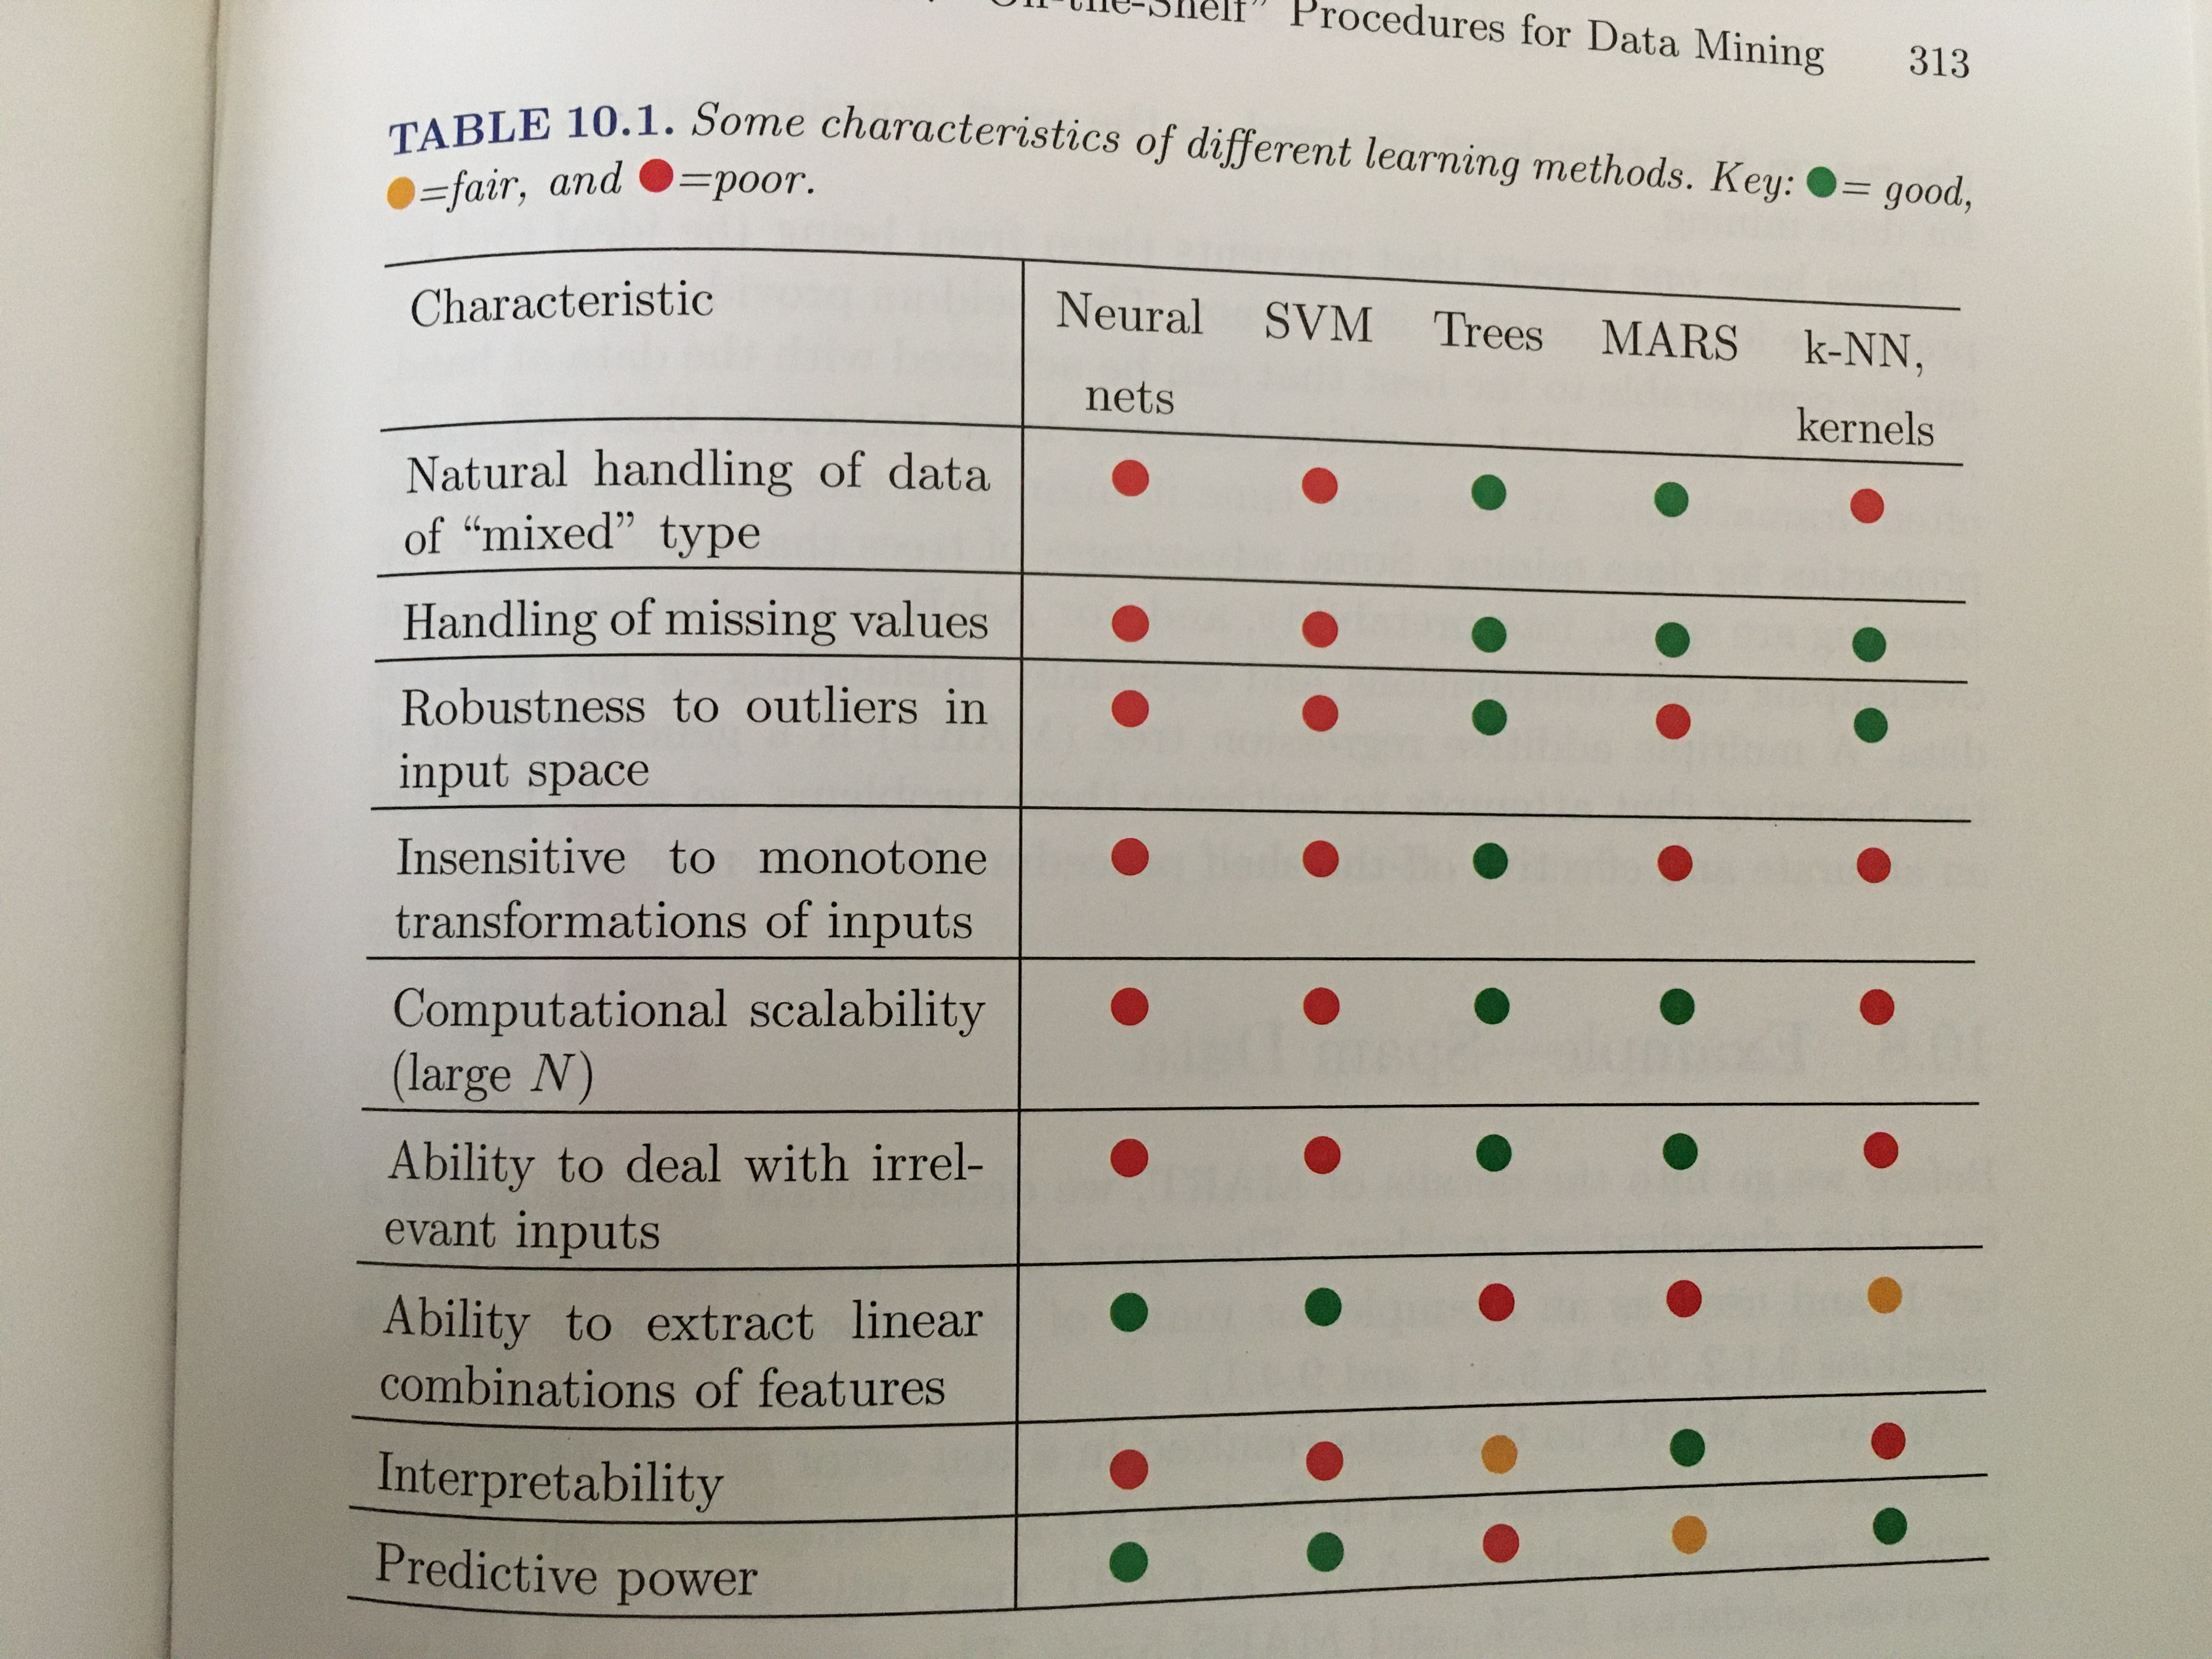
\includegraphics[scale=0.05]{../../Figures/fig_comparison.png}
\end{figure}
\end{frame}

\begin{frame}{References}
	Materials and some of the pictures are from \citep{James2015}, \citep{genuer}, \citep{dubook}, and \citep{hastie01}.
	\printbibliography 	
	
	I have used some of the graphs by hacking TiKz code from StakExchange, Inkscape for more aesthetic plots and other old tricks of \TeX
	
\end{frame}



\end{document}